\documentclass[12pt,letterpaper]{article}

\usepackage[utf8]{inputenc}
\usepackage[spanish]{babel}
\usepackage{graphicx}
\usepackage[hidelinks]{hyperref}
\usepackage{hyperref}
\usepackage[left=2cm,right=2cm,top=2.5cm,bottom=2cm]{geometry}
\usepackage{graphicx}
\usepackage{float}
\usepackage{amsmath}
\usepackage{stackrel} 
\usepackage{multicol}
\usepackage{multirow}
\usepackage{fancyhdr}
\usepackage[usenames,dvipsnames,svgnames,table]{xcolor}
\usepackage[document]{ragged2e}
\usepackage{enumerate}

\usepackage{helvet}

\renewcommand{\labelitemi}{$-$}
\renewcommand{\labelitemii}{$\cdot$}
\newcommand\tab[1][1cm]{\hspace*{#1}}

\renewcommand{\familydefault}{\sfdefault}

\definecolor{azul}{RGB}{0,0,255}

\pagestyle{fancy}
\lhead{\begin{picture}(0,0) \put(0,0){
\includegraphics[width=10mm]{./img/logo}} \end{picture}}
\chead{\hspace{1cm}\vspace{0.2cm}Laboratorio 03 - Dashboards interactivos en Power BI}
\rhead{}

\begin{document}
    \begin{titlepage}
        \begin{center}
            \begin{figure}[htb]
                \begin{center}
                    
\includegraphics[width=3.5cm]{./img/logo}
                \end{center}
            \end{figure}
            \vspace*{0.15in}
            \begin{Large}
                \textbf{UNIVERSIDAD PRIVADA DE TACNA}\\
            \end{Large}
            \vspace*{0.15in}
            \begin{Large}
                \textbf{FACULTAD DE INGENIERÍA} \\
            \end{Large}
            \vspace*{0.1in}
            \begin{Large}
                \textbf{Escuela Profesional de Ingeniería de Sistemas} \\
            \end{Large}
            \vspace*{0.3in}
            \begin{Large}
                \textbf{Laboratorio 03}\\
                \textbf{``Dashboards interactivos en Power BI"}\\
            \end{Large}
            \vspace*{0.2in}
            \begin{Large}
                \textbf{CURSO:} \\
            \end{Large}
            \vspace*{0.1in}
            \begin{large}
                Inteligencia de Negocios\\
            \end{large}
            \vspace*{0.2in}
            \begin{Large}
                \textbf{DOCENTE:} \\
            \end{Large}
            \vspace*{0.1in}
            \begin{large}
                Mag. Patrick Jose Cuadros Quiroga\\
            \end{large}
            \vspace*{0.3in}
            \begin{large}
                \textbf{ALUMNO:} \\
                \begin{flushleft}
                    Lipa Calabilla, Abraham  		\hfill	(2019064039) \\
                \end{flushleft}
            \end{large}
            \vspace*{1.3in}
            \begin{large}
                Tacna - Perú\\
            \end{large}
            \vspace*{0.1in}
            \begin{large}
                2022\\
            \end{large}
        \end{center}
    \end{titlepage}
    \include{Secciones/articulo}
    \newpage
    \tableofcontents
    \justify
    \newpage
    \begin{LARGE}
        \begin{center}
            \textbf{DASHBOARDS INTERACTIVOS EN POWER BI} \\
        \end{center}
    \end{LARGE}
    \section{OBJETIVOS}
    \begin{itemize}
        \item Crear reportes interactivos haciendo uso de las herramientas de Power BI.
    \end{itemize}
    
    \section{REQUERIMIENTOS}
    \begin{itemize}
        \item Conocimientos\\
        Para el desarrollo de esta práctica se requerirá de los siguientes conocimientos básicos:
        \begin{itemize} 
            \item Conocimientos básicos de administración de base de datos Microsoft SQL Server.
            \item Conocimientos básicos de SQL.
        \end{itemize}
        \item Hardware
        \begin{itemize}
            \item CPU SLAT-capable feature.
            \item Al menos 4GB de RAM.
        \end{itemize}
        \item Software\\
        Así mismo se necesitan los siguientes aplicativos
        \begin{itemize}
            \item Microsoft SQL Server 2016 o superior.
            \item Base de datos AdventureWorksLT2016 o superior.
            \item Tener los archivos de recursos del laboratorio.
            \item Power BI Desktop.
            \item Tener una cuenta Microsoft registrada en el Portal de Power Bi.
        \end{itemize}
    \end{itemize}
    
    \section{CONSIDERACIONES INICIALES}
    \begin{itemize}
        \item Generar una carpeta o directorio Power BI en un lugar accesible para guardar los resultados de la práctica.
    \end{itemize}
    
    \newpage
    \section{DESARROLLO}
    
    \subsection{Conexión a datos de Power BI}
    \subsubsection{Conectar a datos existentes}
    \begin{enumerate}[\tab 1.]
        \item Abrir SQL Server Management Studio, y conectar a la instancia de base de datos \textbf{(local)} utilizando autenticación de Windows.
        \item En el menú Archivo \textbf{(File)}, en el submenu Abrir \textbf{(Open)}, hacer click en \textbf{Project/Solution}, y buscar el archivo \textbf{Project.ssmssln}.
        \item En el Explorador de Soluciones, expandir Consultas \textbf{(Queries)}, y luego hacer doble click en el archivo \textbf{Lab Exercise 1.sql}.
        \begin{center}
            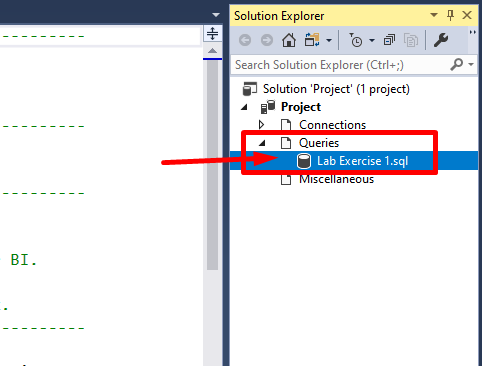
\includegraphics[width=8cm]{./img/img3.png}
        \end{center}
        \item Abrir \textbf{Power BI Desktop}.
        \item En la ventana Power BI Desktop, hacer click en Obtener Data \textbf{(Get Data)}.
        \begin{center}
            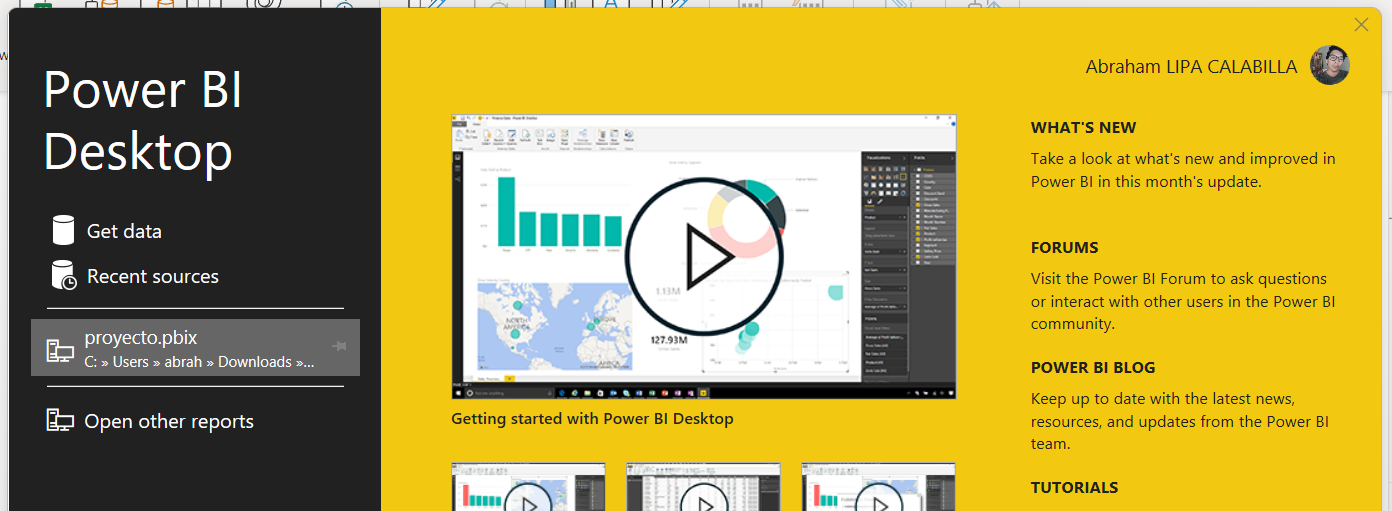
\includegraphics[width=13cm]{./img/img5.png}
        \end{center}
        \item En el cuadro Obtener Datos, click base de datos \textbf{Microsoft SQL}, y entonces click en Conectar.
        \begin{center}
            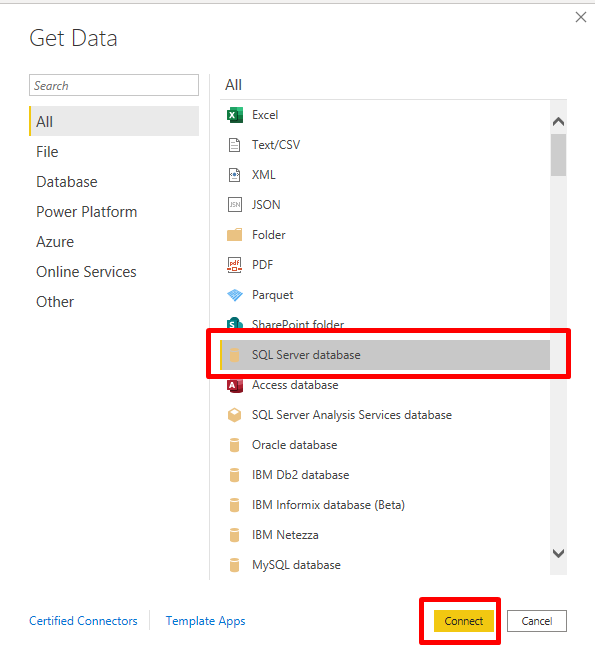
\includegraphics[width=8cm]{./img/img6.png}
        \end{center}
        \item En la ventana base de datos Server database, En \textbf{Servidor}, escribir \textbf{(localhost)}.
        \item En \textbf{Base de Datos (opcional)}, tipear \textbf{AdventureWorksLT2016}.
        \item Expandir el cuadro \textbf{Opciones Avanzadas}. Copiar el script \textbf{Task 1} del archivo \textbf{Lab Exercise 1.sql}. y pegar la consulta en Power BI, en el cuadro sentencia SQL. Luego presionar OK.
        \begin{center}
            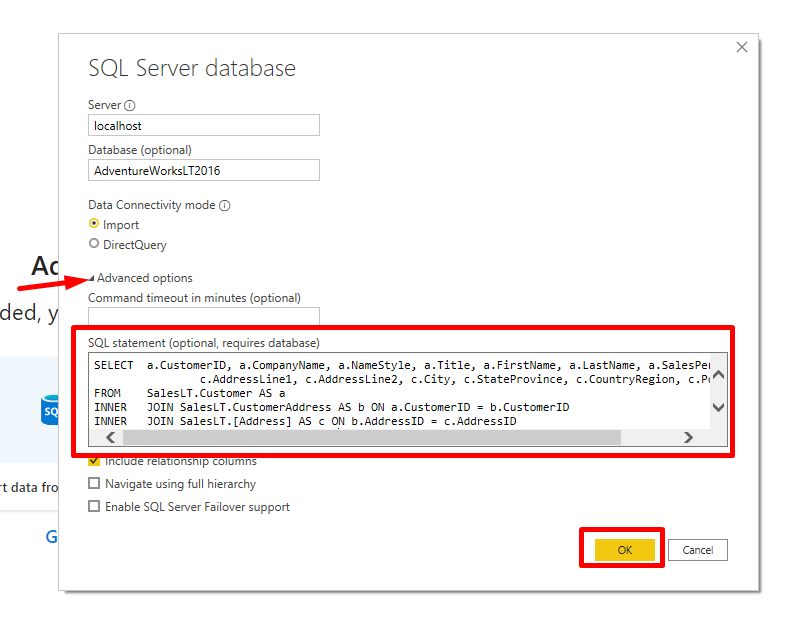
\includegraphics[width=8cm]{./img/img9.png}
        \end{center}
        \item En la ventana de vista prDelete click en \textbf{Load}.
        \item En Power BI Desktop, click \textbf{Obtener Datos} y luego click en Mas.
        \item Repetir los pasos del 6 al 10, utilizando el script \textbf{Task 2}.
        \begin{center}
            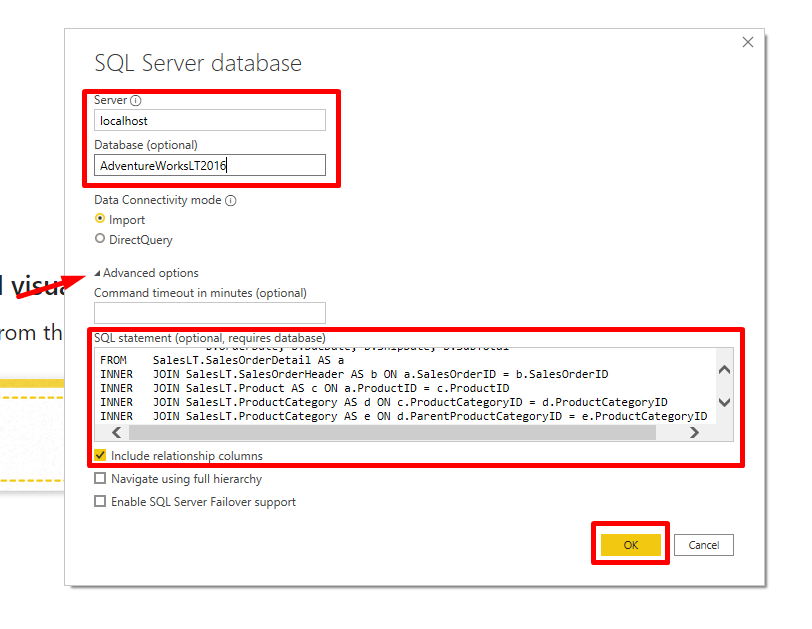
\includegraphics[width=13cm]{./img/img12.png}
        \end{center}
        \item De regreso en el reporte. Guardar el archivo como \textbf{AdventureWorksLT Sales.pbix}.
    \end{enumerate}
    \subsubsection{Graficar Datos}
    \begin{enumerate}[\tab 1.]
        \item En el panel \textbf{Fields} \textbf{(Fields)}, click derecho sobre \textbf{Query1}, clic en \textbf{Rename}, tipear \textbf{Customers} y presionar Enter.
        \item Haga clic con el botón derecho en \textbf{Query2}, haga clic en \textbf{Rename}, escriba \textbf{Sales} y, a continuación, presione Enter.
        \item Expanda las dos tablas para mostrar todos los \textbf{Fields}.
        \begin{center}
            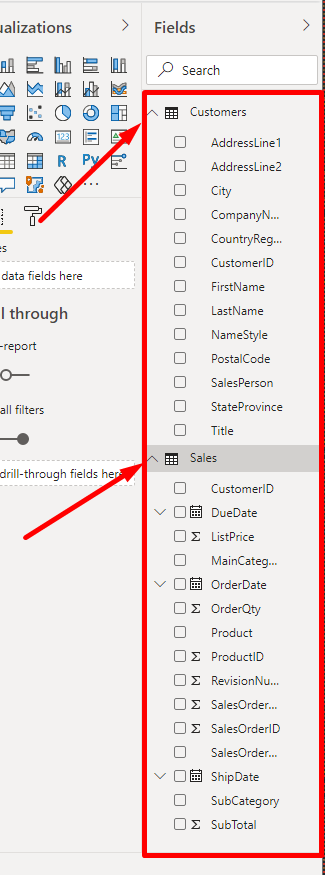
\includegraphics[width=5cm]{./img/img16.png}
        \end{center}
        \item En la barra de navegación izquierda, haga clic en \textbf{Data}.
        \begin{center}
            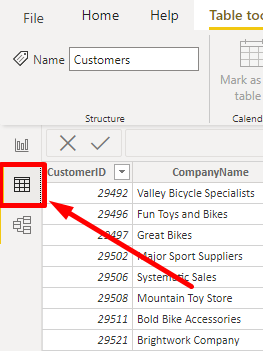
\includegraphics[width=5cm]{./img/img17.png}
        \end{center}
        \item En el panel \textbf{Fields} \textbf{(Fields)}, haga clic en la tabla Customers, si aún no está seleccionada.
        \item Haga clic con el botón derecho en la columna \textbf{NameStyle} y haga clic en \textbf{Delete}.
        \begin{center}
            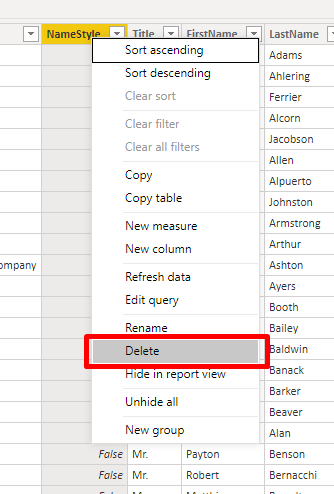
\includegraphics[width=6cm]{./img/img19.png}
        \end{center}
        \item En el cuadro de diálogo \textbf{Delete Column}, haga clic en \textbf{Delete}.
        \item Haga clic con el botón derecho en la columna \textbf{SalesPerson} y haga clic en \textbf{Delete}.
        \item En el cuadro de diálogo \textbf{Delete Column}, haga clic en \textbf{Delete}.
        \item Haga clic con el botón derecho en la columna \textbf{CustomerID} y luego haga clic en \textbf{Hide in ReportView}.
        \begin{center}
            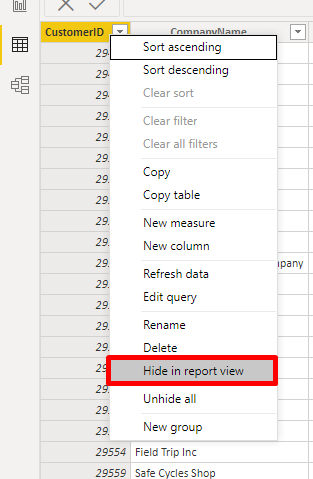
\includegraphics[width=6cm]{./img/img23.png}
        \end{center}
        \item Haga clic en el encabezado de la columna \textbf{AddressLine1}.
        \item En la cinta \textbf{Modeling}, en el grupo \textbf{Properties}, haga clic en \textbf{DataCategory: Uncategorized} y luego en \textbf{Address}.
        \begin{center}
            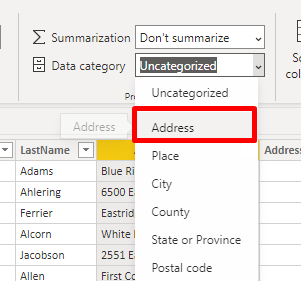
\includegraphics[width=6cm]{./img/img25.png}
        \end{center}
        \item Haga clic en el encabezado de la columna \textbf{City}.
        \item En la cinta de \textbf{Modeling}, en el grupo \textbf{Properties}, haga clic en \textbf{DataCategory: Uncategorized} y, a continuación, haga clic en \textbf{City}.
        \begin{center}
            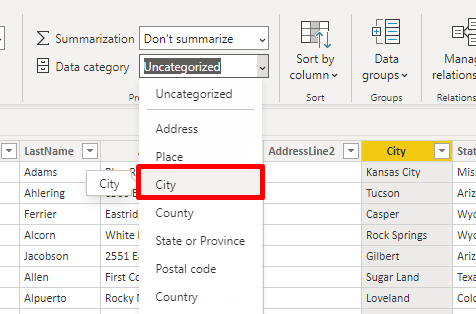
\includegraphics[width=6cm]{./img/img27.png}
        \end{center}
        \item Haga clic en el encabezado de la columna \textbf{StateProvince}.
        \item En la cinta \textbf{Modeling}, en el grupo \textbf{Properties}, haga clic en \textbf{DataCategory: Uncategorized} y luego haga clic en \textbf{State or Province}.
        \begin{center}
            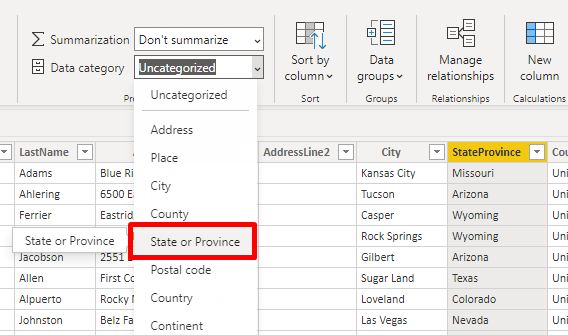
\includegraphics[width=6cm]{./img/img29.png}
        \end{center}
        \item Haga clic en el encabezado de la columna \textbf{CountryRegion}.
        \item En la cinta \textbf{Modeling}, en el grupo \textbf{Properties}, haga clic en \textbf{DataCategory: Uncategorized} y luego haga clic en \textbf{Country}.
        \begin{center}
            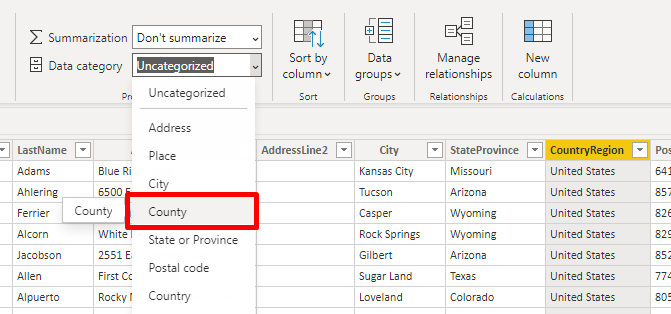
\includegraphics[width=6cm]{./img/img31.png}
        \end{center}
        \item Haga clic en el encabezado de la columna \textbf{PostalCode}.
        \item En la cinta \textbf{Modeling}, en el grupo \textbf{Properties}, haga clic en \textbf{DataCategory: Uncategorized} y luego en \textbf{Postal Code}.
        \begin{center}
            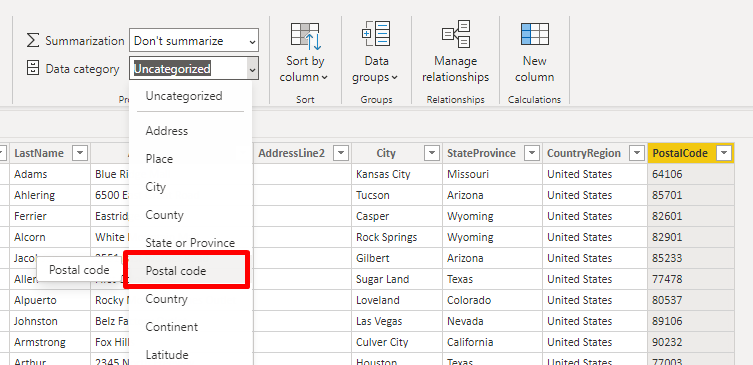
\includegraphics[width=6cm]{./img/img33.png}
        \end{center}
        \item En la cinta \textbf{Modeling}, en el grupo \textbf{Calculations}, haga clic en \textbf{NewColumn} y luego en la barra de fórmulas, escriba la siguiente expresión y presione Enter:
        \begin{center}
            \textbf{FullAddress = Customers[AddressLine1] \& ", " \& Customers[City] \& ", " \& Customers[StateProvince] \& ", " \& Customers[CountryRegion] \& ", " \& Customers[PostalCode]}
            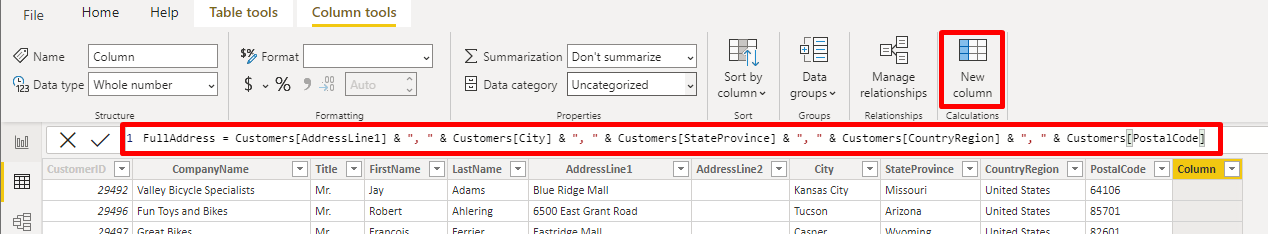
\includegraphics[width=13cm]{./img/img34.png}
        \end{center}
        \item En el panel \textbf{Fields} \textbf{(Fields)}, haga clic en \textbf{Sales}.
        \item Haga clic con el botón derecho en la columna \textbf{RevisionNumber} y haga clic en \textbf{Delete}.
        \begin{center}
            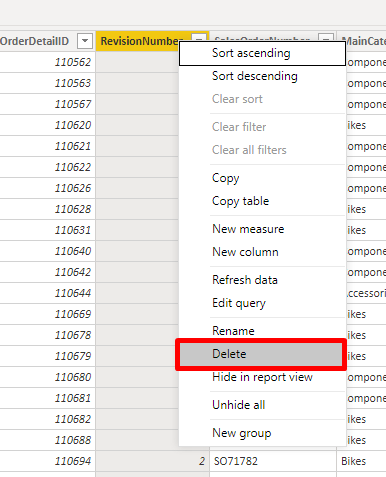
\includegraphics[width=5cm]{./img/img36.png}
        \end{center}
        \item En el cuadro de diálogo \textbf{Delete Column}, haga clic en \textbf{Delete}.
        \item Haga clic con el botón derecho en la columna \textbf{SalesOrderNumber} y haga clic en \textbf{Delete}.
        \begin{center}
            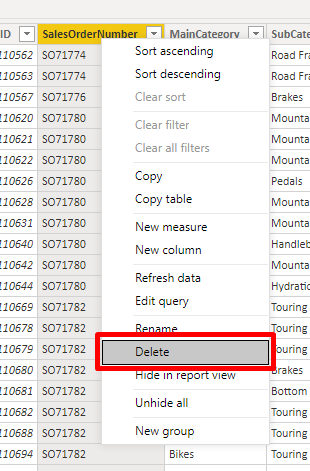
\includegraphics[width=5cm]{./img/img38.png}
        \end{center}
        \item En el cuadro de diálogo \textbf{Delete Column}, haga clic en \textbf{Delete}.
        \item Haga clic con el botón derecho en la columna \textbf{CustomerID} y luego haga clic en \textbf{Hide in ReportView}.
        \begin{center}
            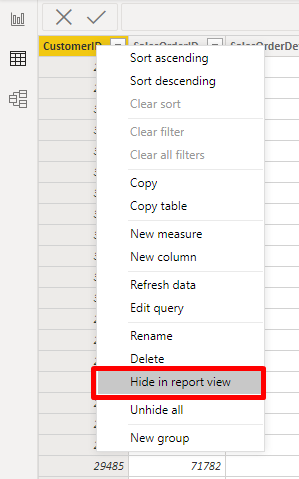
\includegraphics[width=6cm]{./img/img40.png}
        \end{center}
        \item Haga clic con el botón derecho en la columna \textbf{SalesOrderID} y luego haga clic en \textbf{Hide in ReportView}.
        \item Haga clic con el botón derecho en la columna \textbf{SalesOrderDetailID} y luego haga clic en \textbf{Hide in ReportView}.
        \item En la cinta \textbf{Modeling}, en el grupo \textbf{Calculations}, haga clic en \textbf{NewColumn} y luego en la barra de fórmulas, escriba la siguiente expresión y presione Enter:
        \begin{center}
            \textbf{LineTotal = Sales[OrderQty] * Sales[ListPrice]}
            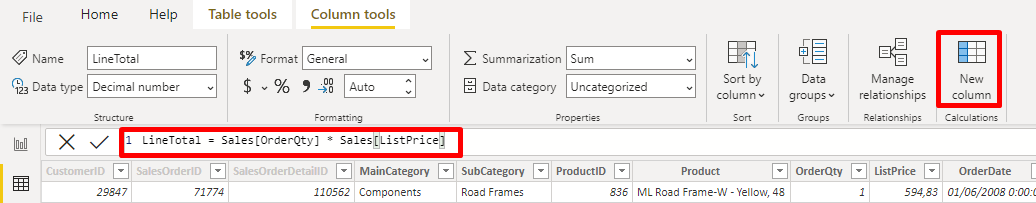
\includegraphics[width=13cm]{./img/img43.png}
        \end{center}
        \item Haga clic en el encabezado de la columna \textbf{LineTotal}.
        \item En la cinta \textbf{Modeling}, en el grupo \textbf{Formatting}, haga clic en \textbf{Format:General}, señale \textbf{Currency} y luego haga clic en \textbf{\$ English (United States)}.
        \begin{center}
            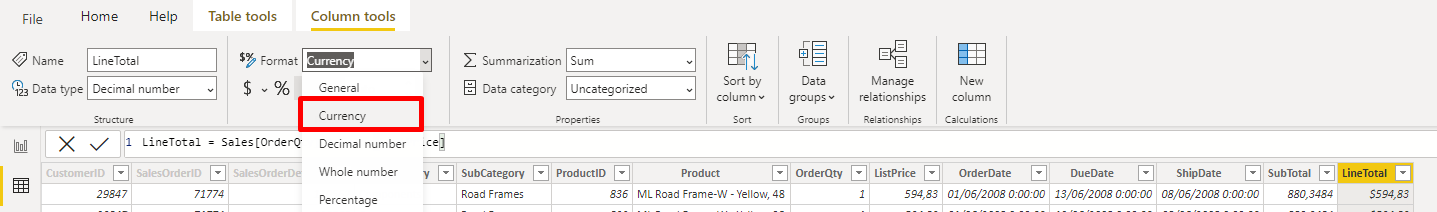
\includegraphics[width=13cm]{./img/img45.png}
        \end{center}
        \item En la cinta \textbf{Modeling}, en el grupo \textbf{Calculations}, haga clic en \textbf{NewMeasure} y luego en la barra de fórmulas, escriba la siguiente expresión y presione Enter.
        \begin{center}
            \textbf{TargetSales = SUM('Sales'[LineTotal]) * 1.2}
            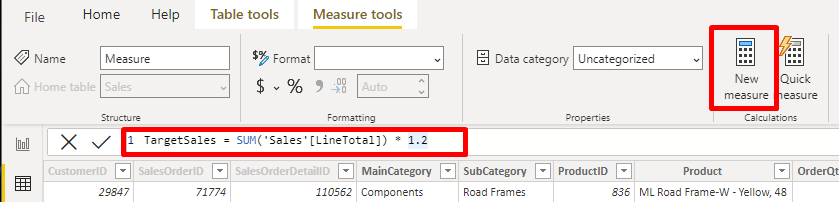
\includegraphics[width=13cm]{./img/img46.png}
        \end{center}
        \item Haga clic en \textbf{Save} y deje Power BI Desktop abierto para la siguiente tarea.
    \end{enumerate}
    \subsubsection{Combinar Data}
    \begin{enumerate}[\tab 1.]
        \item En el \textbf{Explorador de archivos} y luego abra el archivo \textbf{States.xlsx}.
        \item En la hoja de trabajo de \textbf{States}, seleccione todos los valores en las dos columnas y luego presione Ctrl + C.
        \item En Power BI Desktop, en la cinta \textbf{Home}, haga clic en Enter Data.
        \begin{center}
            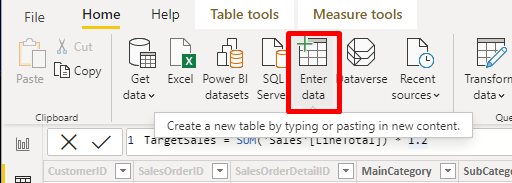
\includegraphics[width=13cm]{./img/img50.png}
        \end{center}
        \item En el cuadro de diálogo Crear tabla, haga clic en la tabla y luego presione Ctrl + V. Power BI detecta que la primera fila es un encabezado de columna.
        \begin{center}
            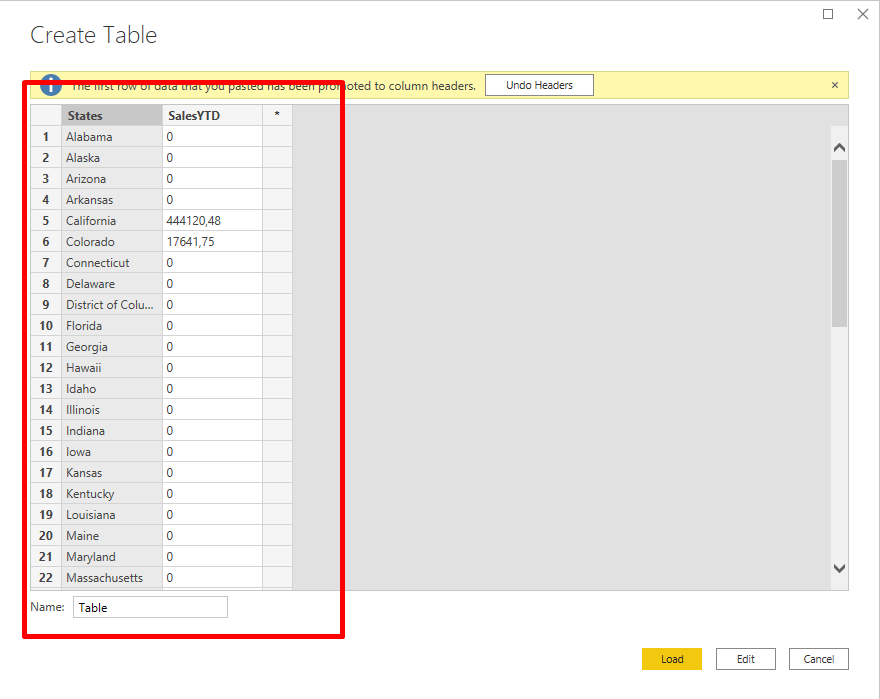
\includegraphics[width=13cm]{./img/img51.png}
        \end{center}
        \item En el cuadro \textbf{Name}, escriba \textbf{Sales by State} y luego haga clic en \textbf{Load}.
        \begin{center}
            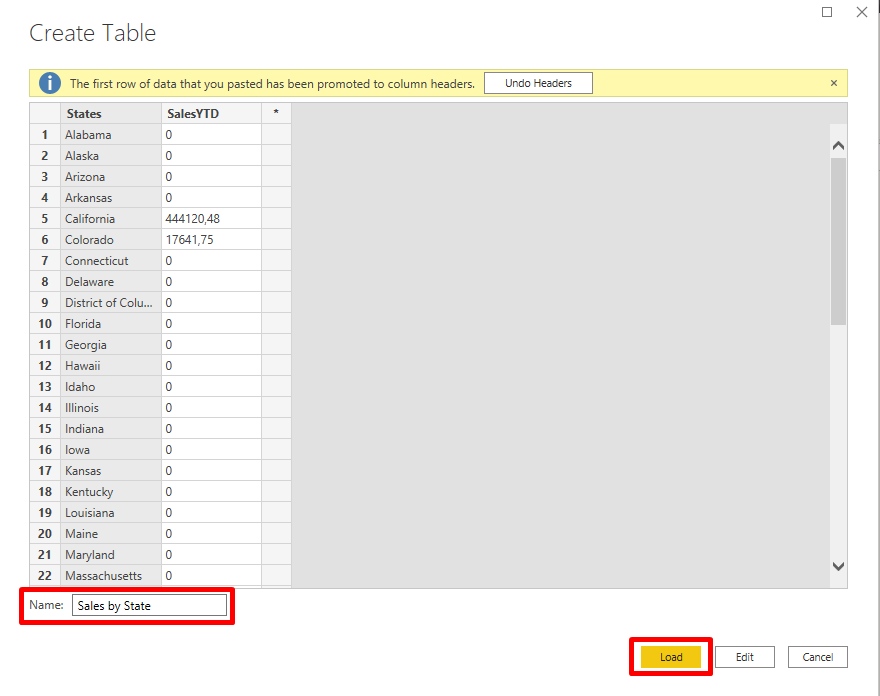
\includegraphics[width=13cm]{./img/img52.png}
        \end{center}
        \item En la cinta \textbf{Home}, haga clic en \textbf{Get Data} y luego en \textbf{Web}.
        \begin{center}
            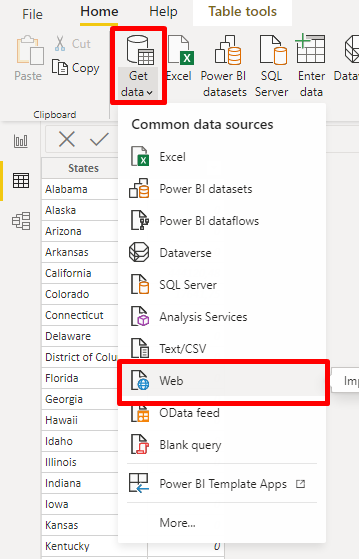
\includegraphics[width=6cm]{./img/img53.png}
        \end{center}
        \item En el cuadro de diálogo \textbf{From Web}, en el cuadro \textbf{URL}, escriba \url{http://en.wikipedia.org/wiki/List_of_U.S._state_abbreviations} y, a continuación, haga clic en \textbf{OK}.
        \item En el cuadro de diálogo \textbf{Navigator}, seleccione \textbf{Codes and abbreviations for U.S. states, territories and other regions}. Y luego haga clic en \textbf{Load}.
        \begin{center}
            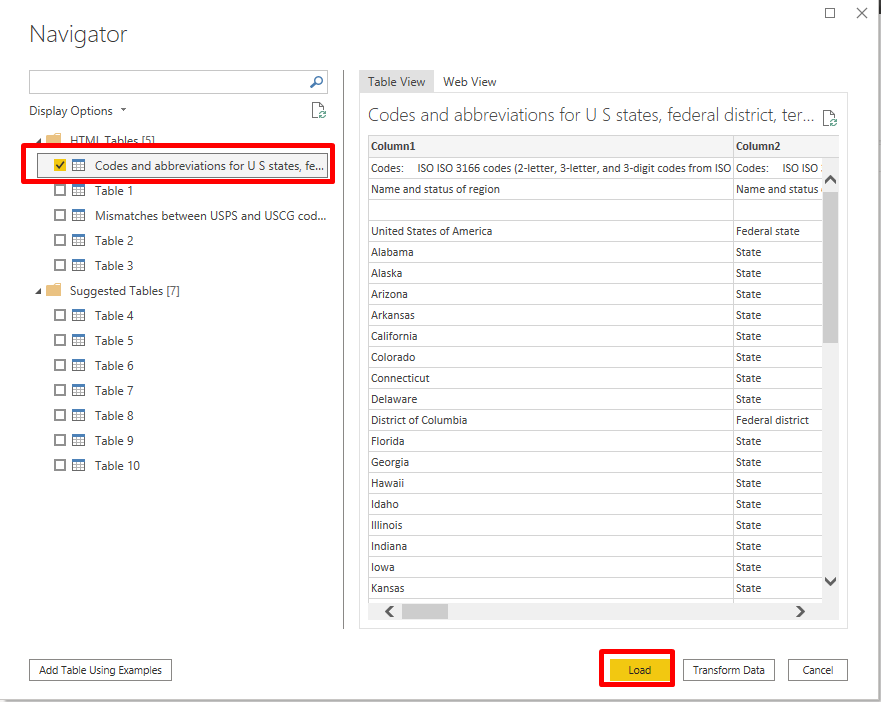
\includegraphics[width=13cm]{./img/img55.png}
        \end{center}
        \item En el panel \textbf{Fields} \textbf{(Fields)}, haga clic en \textbf{Codes and abbreviations for U.S. states, territories and other regions}. Para mostrar los datos. La tabla tiene 26 filas en la parte inferior que no son necesarias.
        \item En la cinta \textbf{Home}, en el grupo \textbf{Queries}, haga clic en \textbf{Transform Data} y luego en \textbf{Transform Data}.
        \begin{center}
            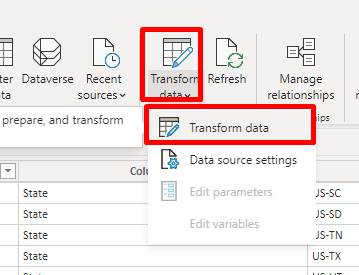
\includegraphics[width=5cm]{./img/img57.png}
        \end{center}
        \item En el Editor de consultas, en el panel \textbf{Query}, haga clic en \textbf{Codes and abbreviations for U.S. states, territories and other regions}.
        \item En la cinta \textbf{Home}, haga clic en \textbf{Reduce Rows}, haga clic en \textbf{Remove Rows} y, a continuación, haga clic en \textbf{Remove Bottom Rows}.
        \begin{center}
            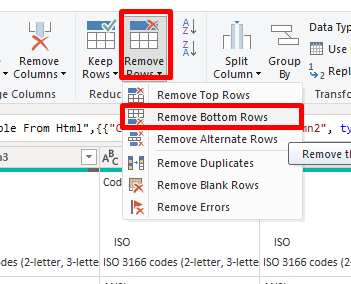
\includegraphics[width=5cm]{./img/img59.png}
        \end{center}
        \item En el cuadro de diálogo \textbf{Remove Bottom Rows}, en el cuadro \textbf{Number of rows}, escriba \textbf{26} y, a continuación, haga clic en \textbf{OK}.
        \item Haga clic en el encabezado de la columna \textbf{ANSI2} y luego mantenga presionada la tecla Ctrl mientras selecciona todas las columnas a la derecha. Esto selecciona varias filas.
        \begin{center}
            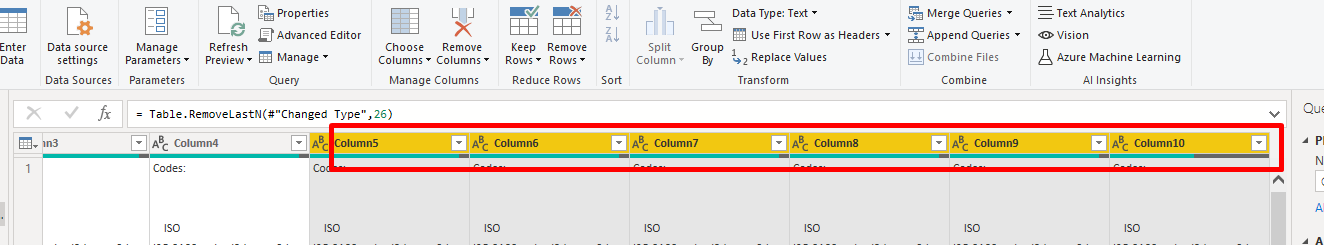
\includegraphics[width=13cm]{./img/img61.png}
        \end{center}
        \item Manteniendo presionada la tecla Ctrl, haga clic en las columnas \textbf{Name and status of region2} y \textbf{Header} para incluir esto en la selección.
        \item En la cinta \textbf{Home}, haga clic en \textbf{Manage Columns}, haga clic en \textbf{Remove Columns} y luego haga clic en \textbf{Remove Columns}.
        \begin{center}
            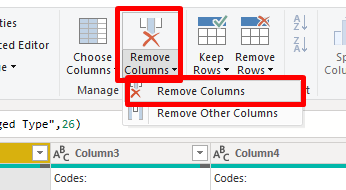
\includegraphics[width=5cm]{./img/img63.png}
        \end{center}
        \item En el panel \textbf{Query Settings}, en \textbf{Properties}, en el cuadro \textbf{Name}, escriba \textbf{States with Codes} y luego presione \textbf{Enter}.
        \begin{center}
            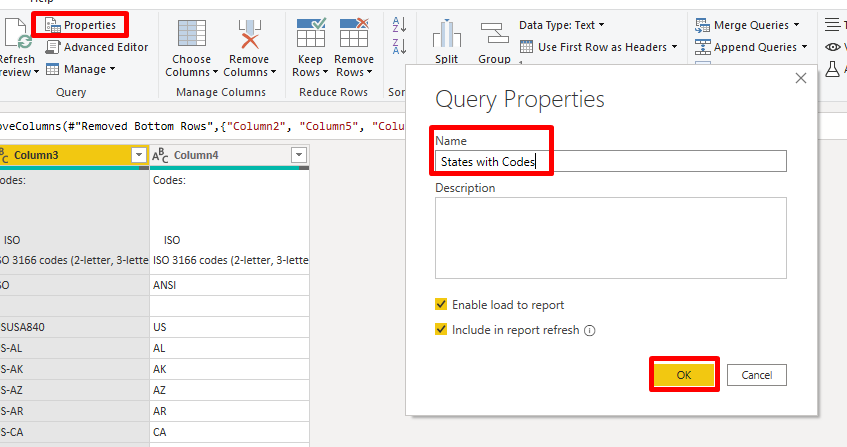
\includegraphics[width=13cm]{./img/img64.png}
        \end{center}
        \item En la cinta \textbf{Home}, en el grupo \textbf{Transform}, haga clic en \textbf{Use First Row as Headers}.
        \item Haga clic con el botón derecho en el encabezado de la columna \textbf{United States of America}, haga clic en \textbf{Rename}, escriba \textbf{State Name} y luego presione Enter.
        \item Haga clic con el botón derecho en el encabezado de la columna \textbf{US USA 840}, haga clic en \textbf{Rename}, escriba \textbf{State Code Long} y luego presione Enter.
        \item Haga clic con el botón derecho en el encabezado de la columna de \textbf{US}, haga clic en \textbf{Rename}, escriba \textbf{State Code Short} y luego presione Enter.
        \item En el panel \textbf{Queries}, haga clic en \textbf{Sales by State}.
        \begin{center}
            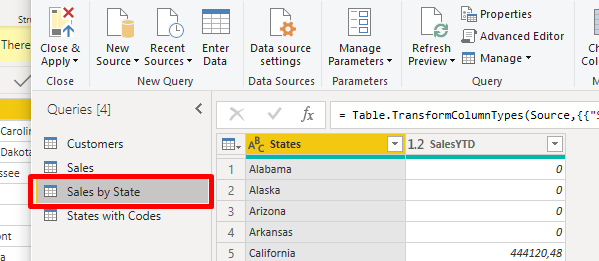
\includegraphics[width=13cm]{./img/img69.png}
        \end{center}
        \item En la cinta \textbf{Home}, haga clic en \textbf{Combine} y luego en \textbf{Merge Queries}.
        \begin{center}
            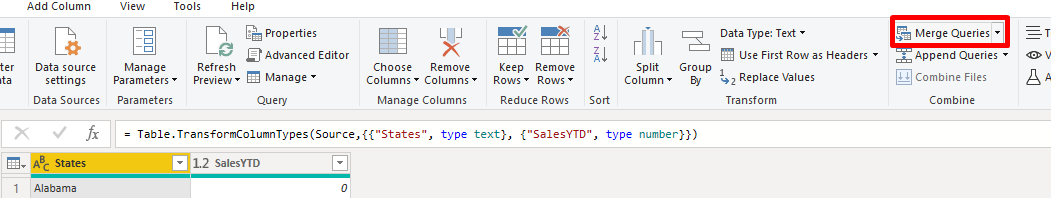
\includegraphics[width=6cm]{./img/img70.png}
        \end{center}
        \item En el cuadro de diálogo \textbf{Merge}, en la tabla \textbf{Sales by State}, haga clic en la columna \textbf{States}.
        \begin{center}
            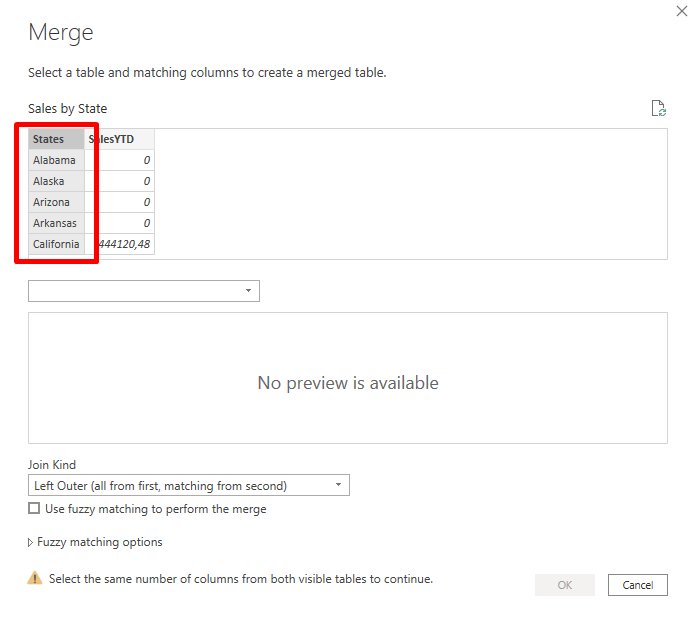
\includegraphics[width=13cm]{./img/img71.png}
        \end{center}
        \item En la lista, haga clic en \textbf{States with Codes}, haga clic en la columna \textbf{State Name} y, a continuación, haga clic en \textbf{OK}. La nueva columna se agrega a la tabla y contiene la tabla \textbf{States with Codes} combinados.
        \begin{center}
            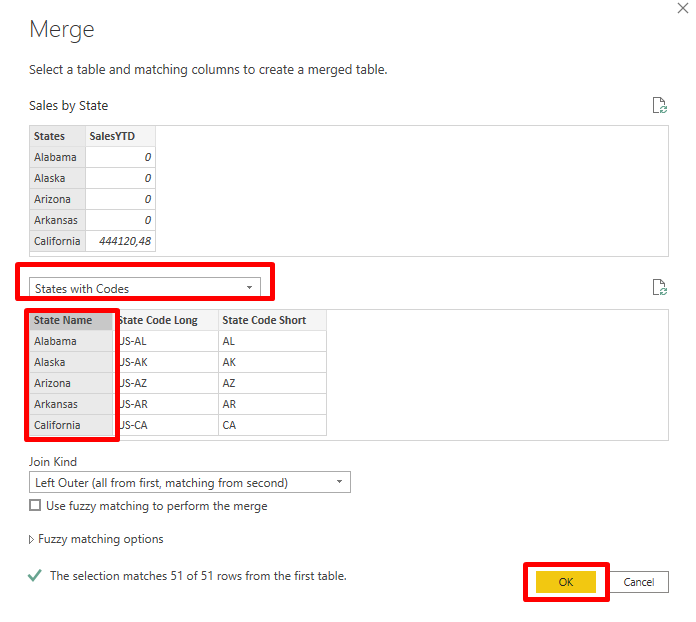
\includegraphics[width=13cm]{./img/img72.png}
        \end{center}
        \item En el encabezado de la columna, haga clic en el icono \textbf{Expand}, desactive \textbf{(Select All Columns)}, seleccione \textbf{State Code Short} y luego haga clic en \textbf{OK}. La columna ahora muestra solo los códigos de estado.
        \begin{center}
            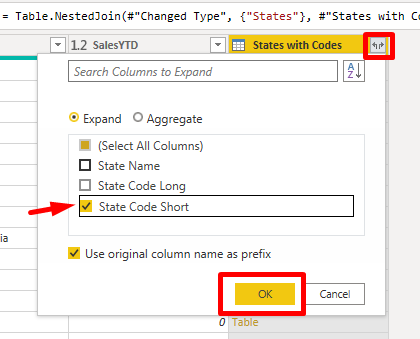
\includegraphics[width=8cm]{./img/img73.png}
        \end{center}
        \item Haga clic con el botón derecho en la columna, haga clic en \textbf{Rename}, escriba \textbf{State Code} y luego presione Enter.
        \item En el menú \textbf{File}, haga clic en \textbf{Close \& Apply}.
        \item En el panel \textbf{Fields} \textbf{(File)}, haga clic con el botón derecho en \textbf{States with Codes} y luego haga clic en \textbf{Hide in Report View}.
        \begin{center}
            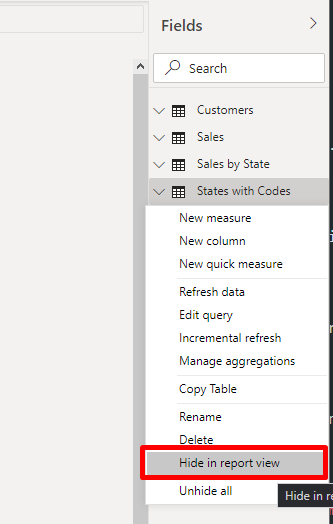
\includegraphics[width=5cm]{./img/img76.png}
        \end{center}
    \end{enumerate}
    
    \subsection{Construyendo Reportes en Power BI}
    \subsubsection{Crear un Gráfico}
    \begin{enumerate}[\tab 1.]
        \item En \textbf{Power BI Desktop}, en la barra de navegación izquierda, haga clic en \textbf{Report}.
        \item En el panel \textbf{Visualizations}, haga clic en \textbf{Gauge}.
        \begin{center}
            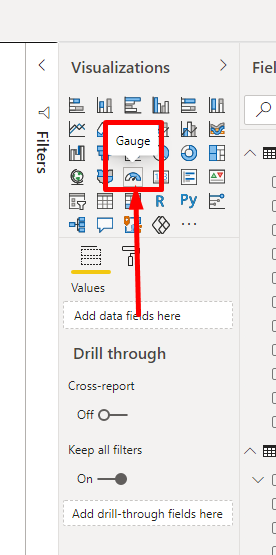
\includegraphics[width=5cm]{./img/img78.png}
        \end{center}
        \item Arrastre el campo \textbf{LineTotal} de la tabla \textbf{Sales} a la propiedad \textbf{Value} del indicador.
        \begin{center}
            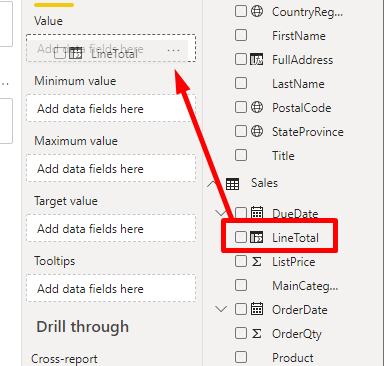
\includegraphics[width=5cm]{./img/img79.png}
        \end{center}
        \item Arrastre la medida \textbf{TargetSales} de la tabla \textbf{Sales} a la propiedad \textbf{Targetvalue} del indicador.
        \begin{center}
            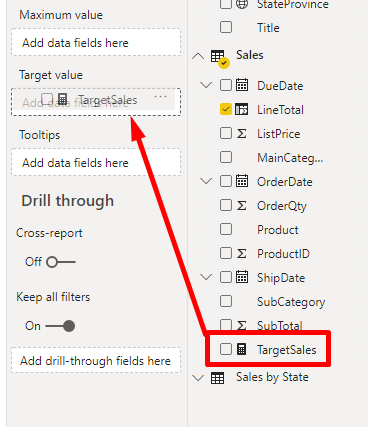
\includegraphics[width=5cm]{./img/img80.png}
        \end{center}
        \item Haga clic en \textbf{Format}, expanda \textbf{Gauge axis} y, a continuación, en el cuadro \textbf{Máx}, escriba \textbf{146000}.
        \begin{center}
            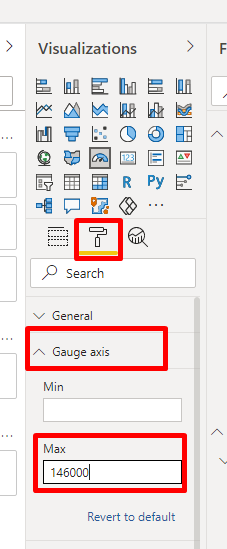
\includegraphics[width=6cm]{./img/img81.png}
        \end{center}
        \item Expanda \textbf{Title}, en el cuadro \textbf{Title Text}, escriba \textbf{Target Sales} y luego haga clic en \textbf{Center}.
        \item Haga clic en el lienzo del informe y luego arrastre el campo \textbf{CompanyName} de la tabla \textbf{Customers} al informe. Power BI crea automáticamente una tabla.
        \item Arrastre el campo \textbf{LineTotal} de la tabla \textbf{Sales} al informe.
        \begin{center}
            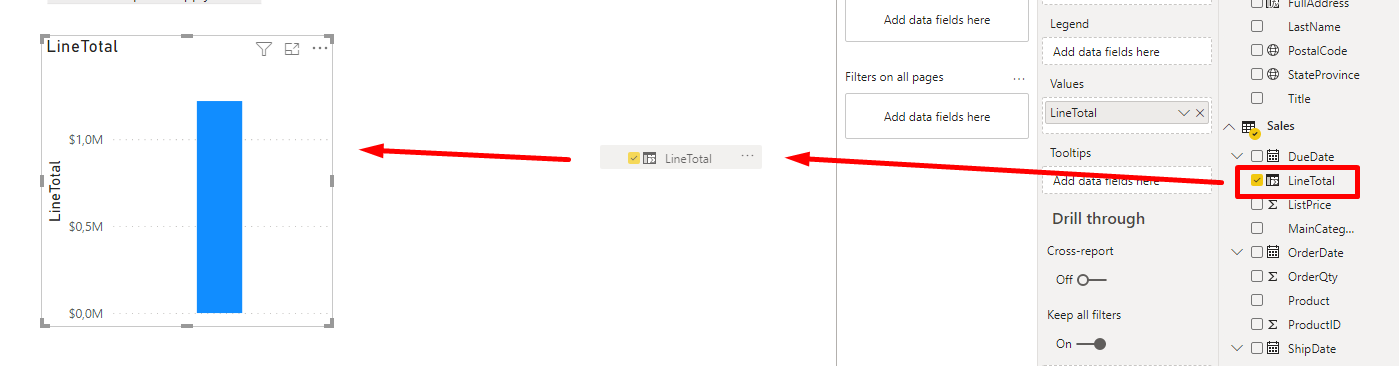
\includegraphics[width=13cm]{./img/img84.png}
        \end{center}
        \item Asegúrese de que la tabla tenga el foco y, a continuación, en el panel \textbf{Visualizations}, haga clic en \textbf{Pie chart}.
        \item Expanda el gráfico para hacer visibles todos los nombres de las empresas utilizando los controladores de tamaño en el borde del gráfico.
        \item Con el foco aún en el gráfico circular, haga clic en \textbf{Format} y luego expanda \textbf{Tilte}.
        \begin{center}
            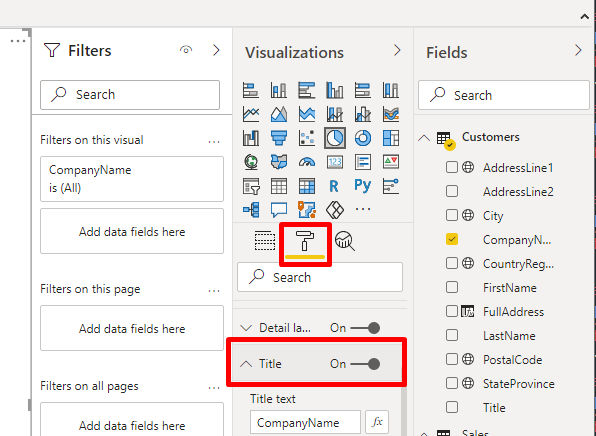
\includegraphics[width=6cm]{./img/img87.png}
        \end{center}
        \item En el cuadro \textbf{Title Text}, escriba Top \textbf{Selling Customers} y luego haga clic en \textbf{Center}.
        \item Arrastre el campo \textbf{MainCategory} de la tabla \textbf{Sales} al panel del informe. Power BI crea una tabla.
        \begin{center}
            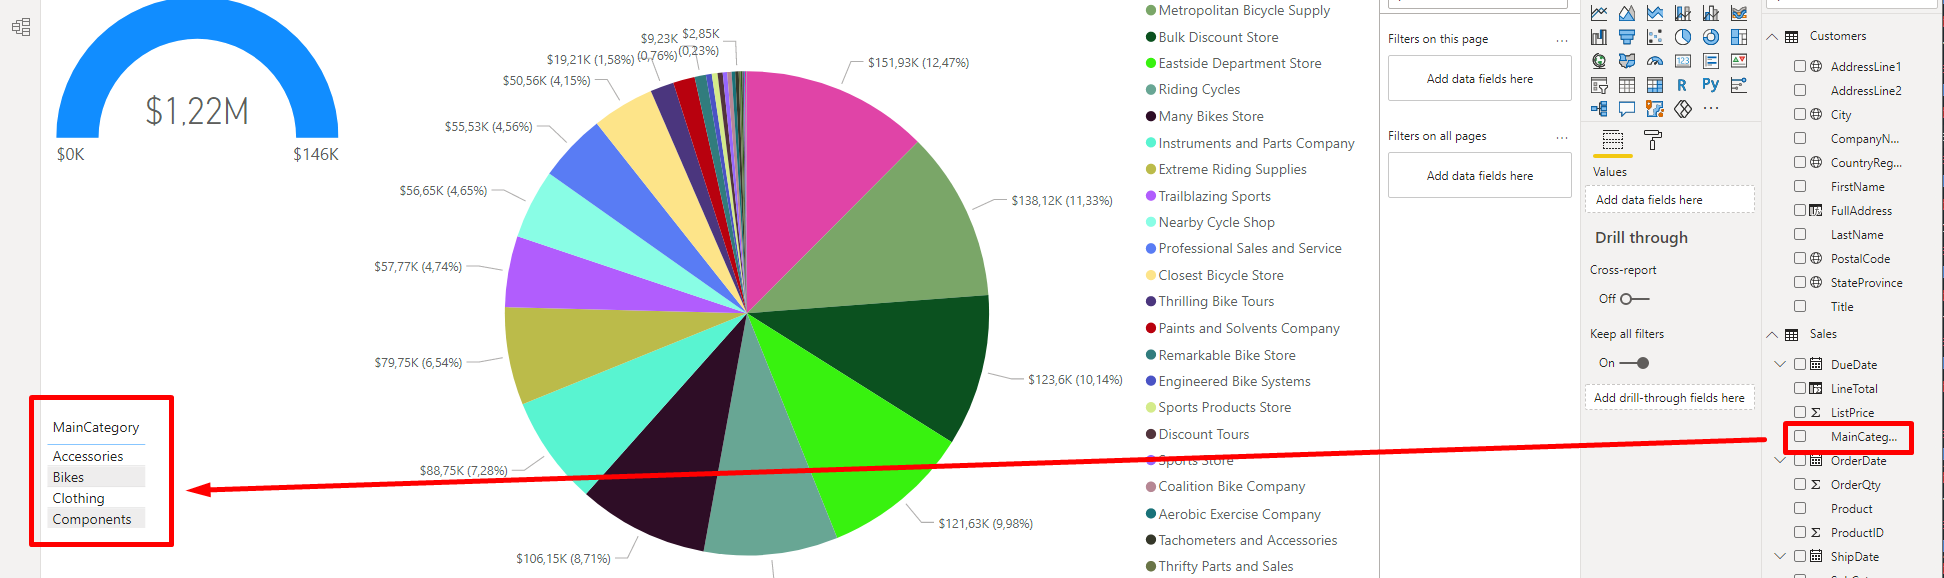
\includegraphics[width=13cm]{./img/img89.png}
        \end{center}
        \item Arrastre el campo \textbf{OrderQty} a la tabla.
        \begin{center}
            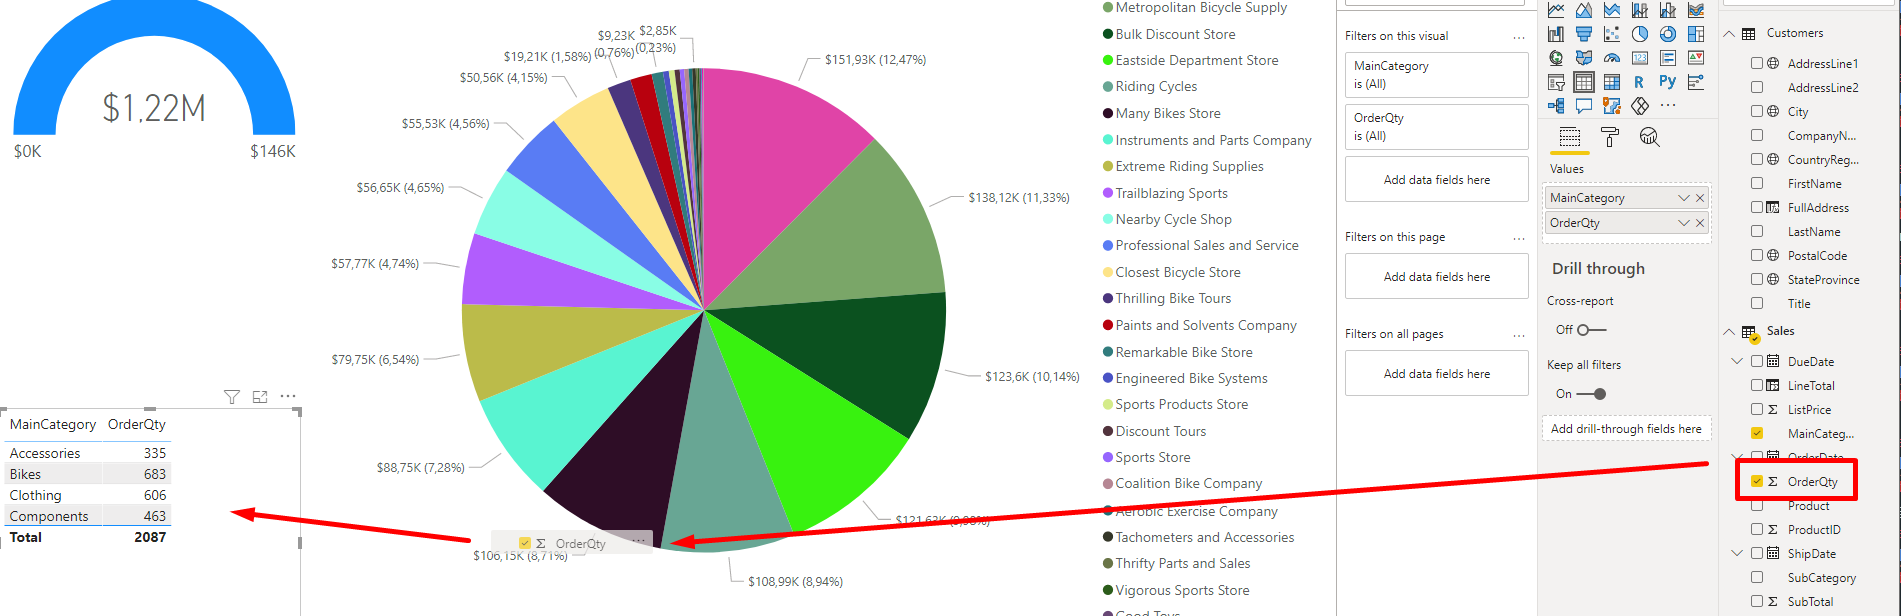
\includegraphics[width=13cm]{./img/img90.png}
        \end{center}
        \item En el panel \textbf{Visualizations}, haga clic en \textbf{Stacked bar chart}.
        \item En el panel \textbf{Visualizations}, haga clic en \textbf{Fields}.
        \item En el panel \textbf{Visualizations}, haga clic en \textbf{Analytics}, expanda \textbf{Constant Line} y luego haga clic en \textbf{Add}.
        \begin{center}
            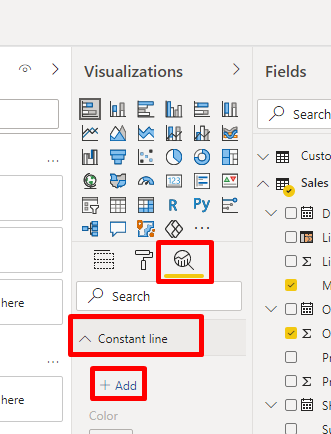
\includegraphics[width=6cm]{./img/img94.png}
        \end{center}
        \item En el cuadro \textbf{Value}, escriba \textbf{500}.
        \item Cambie \textbf{Color} a rojo, cambie \textbf{Data label} a \textbf{On} y luego cambie el color a \textbf{red}.
        \begin{center}
            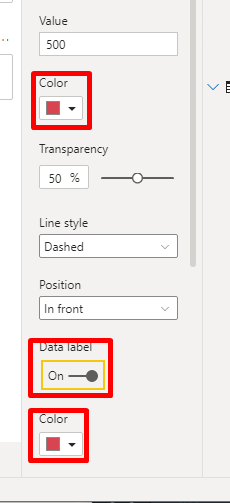
\includegraphics[width=5cm]{./img/img96.png}
        \end{center}
        \item En el panel \textbf{Visualizations}, haga clic en \textbf{Format} y expanda \textbf{Tilte}.
        \item En el cuadro \textbf{Title Text}, escriba \textbf{Orders by Main Category} y luego haga clic en \textbf{Center}.
        \item Haga clic en el lienzo del informe para enfocarlo y, a continuación, en el panel \textbf{Visualizations}, haga clic en \textbf{Donut chart}.
        \begin{center}
            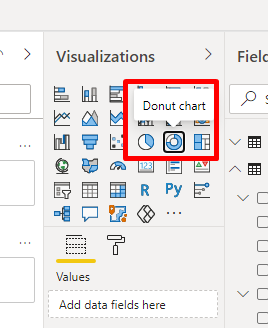
\includegraphics[width=6cm]{./img/img99.png}
        \end{center}
        \item En la tabla \textbf{Sales}, seleccione \textbf{MainCategory} y \textbf{LineTotal}.
        \begin{center}
            \includegraphics[width=13cm]{./img/img100.png}
        \end{center}
        \item En el panel \textbf{Visualizations}, haga clic en \textbf{Format} y luego expanda \textbf{Title}.
        \item En el cuadro \textbf{Title Text}, escriba \textbf{Sales by Main Category} y luego haga clic en \textbf{Center}.
        \item Arrastre el campo \textbf{Product} de la tabla \textbf{Sales} al lienzo del informe. Power BI crea una tabla.
        \item Arrastre el campo \textbf{LineTotal} de la tabla \textbf{Sales} al gráfico de tabla de productos.
        \begin{center}
            \includegraphics[width=13cm]{./img/img104.png}
        \end{center}
        \item En la tabla \textbf{Sales}, seleccione el campo \textbf{MainCategory}.
        \item En el panel \textbf{Visualizations}, haga clic en \textbf{Fields}.
        \begin{center}
            \includegraphics[width=6cm]{./img/img106.png}
        \end{center}
        \item En el panel \textbf{Filters}, expanda \textbf{LineTotal(All)}.
        \item En la lista \textbf{Show items when the value}, seleccione \textbf{is greater than} y, a continuación, en el cuadro siguiente, escriba \textbf{32000}.
        \item Haga clic en \textbf{Apply filter}.
        \item Expanda \textbf{MainCategory(All)} y luego seleccione \textbf{Bikes}.
        \begin{center}
            \includegraphics[width=8cm]{./img/img110.png}
        \end{center}
        \item En el panel \textbf{Visualizations}, haga clic en \textbf{Stacked column chart}.
        \begin{center}
            \includegraphics[width=6cm]{./img/img111.png}
        \end{center}
        \item En el panel \textbf{Visualizations}, haga clic en \textbf{Format} y luego expanda \textbf{Title}.
        \item En el cuadro \textbf{Title Text}, escriba \textbf{Top 10 Selling Bikes1} y luego haga clic en \textbf{Center}.
        \item En el panel \textbf{Visualizations}, haga clic en \textbf{Analytics}, expanda \textbf{Constant Line} y luego haga clic en \textbf{Add}.
        \begin{center}
            \includegraphics[width=6cm]{./img/img114.png}
        \end{center}
        \item En el cuadro \textbf{Value}, escriba \textbf{35000} y luego establezca \textbf{Color} en \textbf{red}.
        \item Cambie \textbf{Data label} a \textbf{On} y luego establezca \textbf{Color} en \textbf{red}.
        \item Expanda el gráfico para llenar el espacio restante en el lienzo del informe. Si es necesario, mueva sus imágenes para que encajen.
        \begin{center}
            \includegraphics[width=13cm]{./img/img117.png}
        \end{center}
        \item Clic en \textbf{Save}.
    \end{enumerate}
    
    \subsubsection{Crear una Visualización de Mapa}
    \begin{enumerate}[\tab 1.]
        \item En la parte inferior del informe, haga clic en el icono + para agregar una nueva página.
        \begin{center}
            \includegraphics[width=6cm]{./img/img119.png}
        \end{center}
        \item En el panel \textbf{Fields}, en la tabla \textbf{Customers}, seleccione el campo \textbf{City}. Power BI agrega un mapa al informe.
        \item En el panel \textbf{Fields}, en la tabla \textbf{Sales}, seleccione el campo \textbf{LineTotal}.
        \begin{center}
            \includegraphics[width=13cm]{./img/img121.png}
        \end{center}
        \item Con la herramienta de captura en el lado derecho del gráfico, cambie el tamaño del mapa para mostrar todas las burbujas.
        \begin{center}
            \includegraphics[width=13cm]{./img/img122.png}
        \end{center}
        \item Observe que las burbujas tienen un tamaño proporcional para representar los datos.
        \item En el panel \textbf{Visualizations}, haga clic en \textbf{Format} y luego expanda \textbf{Title}.
        \item En el cuadro \textbf{Title Text}, escriba \textbf{WorldSales by City} y luego haga clic en \textbf{Center}.
        \item Haga clic en el lienzo del informe y, a continuación, en la tabla \textbf{Sales by State}, seleccione la columna \textbf{State Code}. Power BI agrega automáticamente un mapa.
        \begin{center}
            \includegraphics[width=13cm]{./img/img126.png}
        \end{center}
        \item En la tabla \textbf{Sales by State}, seleccione la columna \textbf{SalesYTD}.
        \item En el panel \textbf{Visualizations}, haga clic en \textbf{Filled Map}. Usando la herramienta de captura en el lado derecho y en la parte inferior del gráfico, cambie el tamaño del mapa para mostrar todos los estados.
        \begin{center}
            \includegraphics[width=6cm]{./img/img128.png}
        \end{center}
        \item Observe que las ventas se agrupan en un área.
        \begin{center}
            \includegraphics[width=13cm]{./img/img129.png}
        \end{center}
        \item Coloque el cursor en \textbf{US-CA} para ver la cifra de ventas. El valor no se ha formateado como moneda.
        \begin{center}
            \includegraphics[width=13cm]{./img/img130.png}
        \end{center}
        \item En el panel \textbf{Fields}, en \textbf{Sales by State}, haga clic en \textbf{SalesYTD}.
        \item En la cinta de \textbf{Modeling}, haga clic en \textbf{Format: General}, señale \textbf{Currency} y luego haga clic en \textbf{\$ English (United Stated)}.
        \begin{center}
            \includegraphics[width=13cm]{./img/img132.png}
        \end{center}
        \item Coloque el cursor en \textbf{US-CA} en el mapa y observe que el valor ha sido formateado.
        \item \textbf{Visualizations}, haga clic en \textbf{Format} y luego expanda \textbf{Title}.
        \item En el cuadro \textbf{Title Text}, escriba \textbf{Sales by State} y luego haga clic en \textbf{Center}.
    \end{enumerate}
    
    \newpage
    \section{CONCLUSIONES}
    \begin{itemize}
        \item La facilidad que tiene ka herramienta para extraer datos de diversas fuentes y despues juntar todos los datos recolectados es impresionante, como se demostro en el presente laboratorio al usar datos de 3 fuentes distintas como son: SQL Server, Excel y una pagina WEB.
        \item Se demostra de que tan facil es hacer reportes interactivos con esta herramienta que tiene una intuitiva interfaz para poder encontrar en los datos aquello que se nos escapa en un análisis convencional mediante consultas a una BD, y animándonos a siempre hacer preguntas adicionales al modelo mediante la selección, y a presentar los datos de diferentes maneras explotando la capacidad y flexibilidad del motor asociativo.
    \end{itemize}
    
    \newpage
    \section{WEBGRAFIA}
    \begin{itemize}
        \item GitHub. (2015). ExploraVisualizaconR.\\
        Recuperado de \textcolor{azul}{\url{https://github.com/fcharte/ExploraVisualizaconR}}
        \item Code Like a Girl. (2018). Análisis y visualización de datos con Pandas \& MatPlotLib.\\
        Recuperado de \textcolor{azul}{\url{https://code.likeagirl.io/analisis-y-visualizacion-de-datos-con-pandas-matplotlib-85ee4d7b4cad}}
        \item Analitics Lane. (2018). Visualización de datos en Python con Seaborn.\\
        Recuperado de \textcolor{azul}{\url{https://www.analyticslane.com/2018/07/20/visualizacion-de-datos-con-seaborn/}}
        \item Microdsosft Docs. (2020). Tutorial de Python: Explorar y visualizar datos.\\
        Recuperado de \textcolor{azul}{\url{https://docs.microsoft.com/es-es/sql/machine-learning/tutorials/python-taxi-classification-explore-data?view=sql-server-2017}}
        \item Hernández, A y Chacón, H. (2019). Manipulación, análisis y visualización de datos de la encuesta demográfica y de salud familiar con el programa R.\\
        Recuperado de \textcolor{azul}{\url{http://www.scielo.org.pe/scielo.php?script=sci_arttext&pid=S1726-46342019000100019&lng=es&nrm=iso&tlng=es}}
        \item GitHub. (2019). Analisis-Endes-Peru.\\
        Recuperado de \textcolor{azul}{\url{https://github.com/horaciochacon/Analisis-Endes-Peru}}
    \end{itemize}
\end{document}